
\chapter{Minimum Weight Perfect Matching}\label{ch:mwpm}


\section{Quasiparticle picture}
The processes of error detection and correction can alternatively be presented in the \emph{quasiparticle picture}, where the anticommuting stabilizer measurements act like excitations on the lattice, which behave like the quasiparticles \emph{anyons}. A single error creates a pair of anyons, and a chain of errors causes movement of the anyon on the lattice. A pair of anyons can also annihilate each other when two error chains merge. The correction of errors can thus be viewed of movement of the correction chains until all anyons are annihilated. The quasiparticle picture removes the distracting underlying lattice from the problem, and decoding becomes simply identifying the right pairing between anyons to minimize the chance of a logical error.
\tikzstyle{rednode}=[circle, fill=red!50, minimum size=4]
\tikzstyle{bluenode}=[circle, fill=cyan!50, minimum size=4]
\tikzstyle{redline}=[red!50, line width = 2]
\tikzstyle{blueline}=[cyan!50, line width = 2]
\tikzstyle{legend}=[anchor=west, font=\small]

\newcommand{\drawquasigrid}{
  \draw[step=.4cm, opacity=.25] (0,0) grid (4,4);
  \draw (0,0) rectangle (4,4);
  \node[rednode] (N1) at (0.5,0.4) {};
  \node[rednode] (N2) at (2,0.7) {};
  \node[rednode] (N3) at (2.5,1.2) {};
  \node[rednode] (N4) at (3.6,1) {};
  \node[rednode] (N5) at (0.75,2.1) {};
  \node[rednode] (N6) at (1.95,1.8) {};
  \node[bluenode] (N7) at (1.6, 3.4) {};
  \node[bluenode] (N8) at (2.7, 3.5) {};
  \node[bluenode] (N9) at (3.2, 2.2) {};
  \node[bluenode] (N10) at (3.1, 0.6) {};
  \draw[blueline] (N1) to[in=170, out=20] (N2);
  \draw[blueline] (N3) to[in=180, out=-10] (N4);
  \draw[blueline] (N5) to[in=170, out=-20] (N6);
  \draw[redline] (N7) to[in=160, out=15] (N8);
  \draw[redline] (N9) to[in=90, out=250] (N10);
}
\begin{figure}
    \centering
    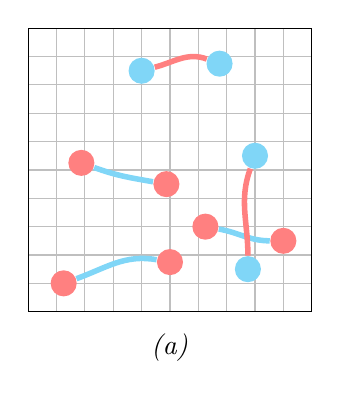
\begin{tikzpicture}[scale=0.9]
      \drawquasigrid
      \node at (2, -.5) {\emph{(a)}};
    \end{tikzpicture}
    \hspace{.3cm}
    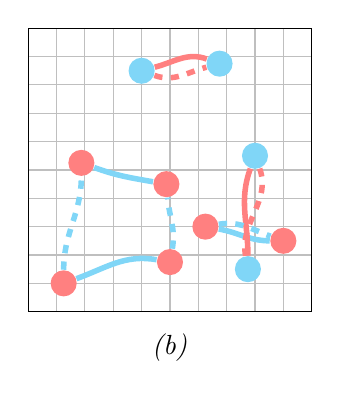
\begin{tikzpicture}[scale=0.9]
      \drawquasigrid
      \draw[dashed, blueline] (N1) to[out=90, in=270] (N5);
      \draw[dashed, blueline] (N2) to[out=80, in=275] (N6);
      \draw[dashed, blueline] (N3) to[out=10, in=160] (N4);
      \draw[dashed, redline] (N7) to[out=-20, in=195] (N8);
      \draw[dashed, redline] (N9) to[out=290, in=100] (N10);
      \node at (2, -.5) {\emph{(b)}};
    \end{tikzpicture}
    \hspace{.3cm}
    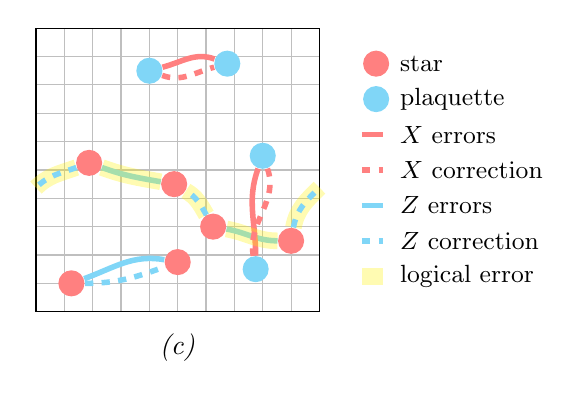
\begin{tikzpicture}[scale=0.9]
      \drawquasigrid
      \draw[yellow, line width=6, opacity=.3] (N3) to[in=180, out=-10] (N4);
      \draw[yellow, line width=6, opacity=.3] (N5) to[in=170, out=-20] (N6);
      \draw[yellow, line width=6, opacity=.3] (N3) to[out=120, in=-30] (N6);
      \draw[yellow, line width=6, opacity=.3] (N5) to[out=200, in=45] (0, 1.75);
      \draw[yellow, line width=6, opacity=.3] (N4) to[out=80, in=225] (4, 1.75);
      \draw[dashed, blueline] (N1) to[out=0, in=200] (N2);
      \draw[dashed, blueline] (N3) to[out=120, in=-30] (N6);
      \draw[dashed, blueline] (N5) to[out=200, in=45] (0, 1.75);
      \draw[dashed, blueline] (N4) to[out=80, in=225] (4, 1.75);
      \draw[dashed, redline] (N7) to[out=-20, in=195] (N8);
      \draw[dashed, redline] (N9) to[out=290, in=100] (N10);
      \node at (2, -.5) {\emph{(c)}};


      \node[rednode] at (4.8, 3.5){};
      \node[bluenode] at (4.8,3){};
      \draw[redline] (4.6,2.5) -- +(0.3,0);
      \draw[redline, dashed] (4.6,2) -- +(0.3,0);
      \draw[blueline] (4.6,1.5) -- +(0.3,0);
      \draw[blueline, dashed] (4.6,1) -- +(0.3,0);
      \draw[yellow, line width=6, opacity=.3] (4.6,.5) -- +(0.3,0);
      \path (5,3.5) node[legend] {star} ++(0,-.5) node[legend] {plaquette} ++(0,-.5) node[legend] {$X$ errors} ++(0,-.5) node[legend] {$X$ correction} ++(0,-.5) node[legend] {$Z$ errors} ++(0,-.5) node[legend] {$Z$ correction} ++(0,-.5) node[legend] {logical error} ;
    \end{tikzpicture}
    \caption{The quasiparticle picture of stabilizer measurements. Anticommuting stabilizers behave as anyons (circles), where a chain of errors (lines) creates a pair of anyons. Figure (b) shows a successful decoding of (a). Figure (c) shows a pairing that resulted in a correction operator that is in a different class as the error operator, which acquires a logical error. (Figure inspired by \cite{naomi})}\label{fig:quasiparticle}
  \end{figure}
  
Figure \ref{fig:quasiparticle}a shows the quasiparticle representation of the errors suffered in Figure \ref{sf:fig_degenerate}a, which has suffered Z (blue lines) and X errors (red lines). The corresponding anyons can either be of the star type (red circle) or plaquette type (blue circle). Figure \ref{fig:quasiparticle}b shows a successful decoding. Note that here not all pairs are correctly identified, but the resulting loop still is in the same class of operators. In Figure \ref{fig:quasiparticle}c the correction has failed as the resulting loop in the correction is in a difference class compared to the error. As the loop still commutes with the stabilizer, no error can be detected, but the encoded qubit has acquired a logical error.

\tikzstyle{rednode}=[circle, fill=red!50, minimum size=1.5]
\tikzstyle{line}=[line width=1]
\tikzstyle{node}=[midway, font=\footnotesize]
\newcommand{\drawmwpmgrid}{
  \draw[step=.4cm, opacity=.25] (-.4,-.4) grid (4.4,4.4);
  \draw (-.4,-.4) rectangle (4.4,4.4);
  \node[rednode] (1) at (0.5,0.4)  {};
  \node[rednode] (2) at (2,0.7)    {};
  \node[rednode] (3) at (2.5,1.2)  {};
  \node[rednode] (4) at (4,1)      {};
  \node[rednode] (5) at (0.75,2.1) {};
  \node[rednode] (6) at (1.95,2.4) {};
  \node[rednode] (7) at (1.6, 3.4) {};
  \node[rednode] (8) at (2.7, 3.5) {};
}
\begin{figure}[htbp]
    \centering
    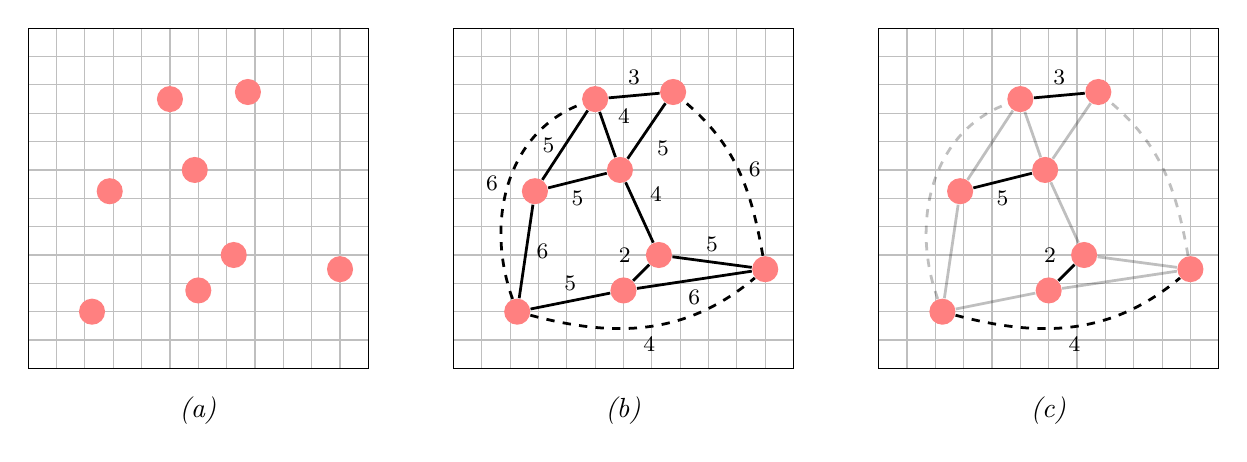
\begin{tikzpicture}[scale=0.9]
      \drawmwpmgrid
      \node at (2,-1) {\emph{(a)}};
    
      \begin{scope}[shift={(6,0)}]
        \drawmwpmgrid
        \draw[line] (2) -- (1) node[node,above]{5} -- (5) node[node, right]{6} -- (6) node[node, below]{5} -- (7) node[node, above right]{4} -- (8) node[node, above]{3} -- (6) node[node, below right]{5};
        \draw[line] (2) -- (3) node[node, above left]{2} -- (4) node[node, above]{5} -- (2) node[node, below]{6};
        \draw[line] (6) -- (3) node[node,above right]{4};
        \draw[line] (5) -- (7) node[node, left]{5};
        \draw[line, dashed] (1) to [out=-15, in=220] node[node,below]{4} (4);
        \draw[line, dashed] (4) to [out=100, in=-40] node[node,right]{6} (8);
        \draw[line, dashed] (1) to [out=110, in=200] node[node,left]{6} (7);
        \node at (2,-1) {\emph{(b)}};

      \end{scope}
      
      \begin{scope}[shift={(12,0)}]
        \drawmwpmgrid
        \draw[line, opacity=.25] (6) -- (3) -- (4) -- (2) -- (1);
        \draw[line, opacity=.25] (1) -- (5) -- (7) -- (6) -- (8) ;
        \draw[line] (7) -- (8) node[node, above]{3};
        \draw[line] (5) -- (6) node[node, below]{5};
        \draw[line] (2) -- (3) node[node, above left]{2};
        \draw[line, dashed] (1) to [out=-15, in=220] node[node,below]{4} (4);
        \draw[line, dashed, opacity=.25] (4) to [out=100, in=-40] (8);
        \draw[line, dashed, opacity=.25] (1) to [out=110, in=200] (7);
        \node at (2,-1) {\emph{(c)}};

      \end{scope}
    \end{tikzpicture}
    \caption{Visualizing the graph matching problem of minimum-weight pairs between anyons. (a) The set of anyons from the measured syndrome are the nodes in the graph matching problem. (b) The graph is initiated by connecting all nodes in the graph with edges weighted correspondingly to the shortest distance between the anyons. High weight edges have been excluded here for clarity. (c) The minimum-weight subset of edges is the result. This figure is inspired by others \cite{naomi2016thesis}.}\label{fig:mwpm}
  \end{figure}
  

\section{Performance}



\begin{table}[htpb]
  \centering
  \begin{tabularx}{\textwidth} { | R{1} || C{1.5} | C{.5} | C{1.5} | C{.5} | }
   \hline
   & \multicolumn{2}{c|}{Independent noise}& \multicolumn{2}{c|}{Phenomenal noise} \\
   \hline
   & $p_{th}$ & $k_C$ & $p_{th}$ & $k_C$ \\
   \hhline{|=#=|=|=|=|}
   Toric code & $0.10349 \pm 0.00004$ & $0.7158$ & $0.02965 \pm 0.00003$ & $0.9024$ \\
   \hline
   Planar code  & $0.10292 \pm 0.00005$ & $0.8478$ & $0.02928 \pm 0.00003$ & $0.928$ \\
  \hline
  \end{tabularx}
  \caption{Simulation results for the Minimum-Weight Perfect Matching decoder $L = 8:8:64, L=8:2:22$}\label{tab:mwpm}
\end{table}
